%%% Econ711: Microeconomics I
%%% Fall 2020
%%% Danny Edgel
%%%
% Due on Canvas Monday September 14, 11:59pm Central Time
%%%

%%%
%							PREAMBLE
%%%

\documentclass{article}

%%% declare packages
\usepackage{amsmath}
\usepackage{amssymb}
\usepackage{array}
\usepackage{bm}
\usepackage{changepage}
\usepackage{centernot}
\usepackage{graphicx}
\usepackage{fancyhdr}
	\fancyhf{} % sets both header and footer to nothing
	\renewcommand{\headrulewidth}{0pt}
    \rfoot{Edgel, \thepage}
    \pagestyle{fancy}
	
%%% define shortcuts for set notation
\newcommand{\N}{\mathbb{N}}
\newcommand{\Z}{\mathbb{Z}}
\newcommand{\R}{\mathbb{R}}
\newcommand{\Q}{\mathbb{Q}}
\newcommand{\lmt}{\underset{x\rightarrow\infty}{\text{lim }}}
\newcommand{\neglmt}{\underset{x\rightarrow-\infty}{\text{lim }}}
\newcommand{\zerolmt}{\underset{x\rightarrow 0}{\text{lim }}}
\newcommand{\usmax}{\underset{1\leq k \leq n}{\text{max }}}

%%% define column vector command (from Michael Nattinger)
\newcount\colveccount
\newcommand*\colvec[1]{
        \global\colveccount#1
        \begin{pmatrix}
        \colvecnext
}
\def\colvecnext#1{
        #1
        \global\advance\colveccount-1
        \ifnum\colveccount>0
                \\
                \expandafter\colvecnext
        \else
                \end{pmatrix}
        \fi
}

%%% define function for drawing matrix augmentation lines
\newcommand\aug{\fboxsep=-\fboxrule\!\!\!\fbox{\strut}\!\!\!}

\makeatletter
\let\amsmath@bigm\bigm

\renewcommand{\bigm}[1]{%
  \ifcsname fenced@\string#1\endcsname
    \expandafter\@firstoftwo
  \else
    \expandafter\@secondoftwo
  \fi
  {\expandafter\amsmath@bigm\csname fenced@\string#1\endcsname}%
  {\amsmath@bigm#1}%
}


%________________________________________________________________%

\begin{document}

\title{	Problem Set \#1 }
\author{ 	Danny Edgel 					\\ 
			Econ 711: Microeconomics I		\\
			Fall 2020						\\
		}
\maketitle\thispagestyle{empty}

\textit{Collaborated with Sarah Bass, Emily Case, Michael Nattinger, and Alex Von Hafften}

%%%________________________________________________________________%%%

\section*{Question 1}
Let $Y\subset R^k$, where, for $y=(y_1,y_2,y_3)\in Y\Rightarrow y_1,y_2\leq0$.
\begin{itemize}
	\item[(a)] \textbf{If} $\mathbf{p_3}$ \textbf{falls and} $\mathbf{p_1}$ \textbf{and} $\mathbf{p_2}$ \textbf{stay the same, can the firm's output} ($\mathbf{y_3}$) \textbf{go up?}
		\smallskip \\
		No. By the Weak Axiom of Profit Maximization (WAPM), if $p,p'\in\R^k$, $y\in Y^*(p)$, and $Y^*(p')$, then $(p'-p)\cdot(y'-y)\geq0$. thus, in our situation, where $p'-p=(0,0,\Delta p_3)$, $\Delta p_3<0$ we can derive:
		\begin{align*}
			(p'-p)\cdot(y'-y) 										&\geq 0 \\														
			(0,0,\Delta p_3)\cdot(\Delta y_1,\Delta y_2,\Delta y_3)	&\geq 0 \\	
			0 + 0 + \Delta p_3 \Delta y_3 							&\geq 0 \\
			\Delta p_3 \Delta y_3 									&\geq 0 
		\end{align*}
		Where $\Delta p_3<0$ by construction. 
		\smallskip \\
		$\therefore$ $\Delta y_3 > 0$ would violate the WAPM and cannot occur $\blacksquare$
		
	\item[(b)] \textbf{If} $\mathbf{p_1}$ \textbf{rises and} $\mathbf{p_2}$ \textbf{and} $\mathbf{p_3}$ \textbf{stay the same, can the firm's output} ($\mathbf{y_3}$) \textbf{go up?}
		\smallskip \\
		Yes. Let $Y=\{y_1,y_2\}=\{(-1,-3,4),(-3,-1,3)\}$ and $p=(1,3,2)$. Then,
		\[
			y(p) = \underset{y\in Y}{\text{argmax }}\{p\cdot y_1,p\cdot y_2\} = \underset{y\in Y}{\text{argmax }}\{-2,0\} 
		\]
		So $y(p)=y_2$. Suppose only $p_1$ rises such that $p'=(3,3,2)$. Then,
		\[
			y(p') = \underset{y\in Y}{\text{argmax }}\{p'\cdot y_1,p'\cdot y_2\} = \underset{y\in Y}{\text{argmax }}\{-4,-6\} 
		\]
		Thus, $y(p')=y_1$, where $y_1$ has a greater output.
		
	\item[(c)]\textbf{If} $\mathbf{p_1}$ \textbf{and} $\mathbf{p_2}$ \textbf{both increase and} $\mathbf{p_3}$ \textbf{stays the same, can the firm's output} ($\mathbf{y_3}$) \textbf{go up? What if} $\mathbf{p_1}$ \textbf{and} $\mathbf{p_2}$ \textbf{both increase by 10\%?}
		\smallskip \\
		It is possible for both $p_1$ and $p_2$ to increase while $y_3$ also increases. Let $Y=\{y,y'\}=\{(-1,-4,5),(-10,-1,10)\}$ and suppose that $p=(1,1,1)$ and $p'=(2,5,1)$. Then:
		\begin{align*}
			p\cdot y		&= -1-4+5 		= 0		\\
			p\cdot y' 	&= -10-1+10 	= -1	\\
			p'\cdot y 	&= -2-20+5		= -17	\\
			p'\cdot y'	&= -20-5+10		= -15	\\
		\end{align*}
		Thus, $y(p)=y$ and $y(p')=y'$, where $y_3<y'_3$.
		\medskip \\
		It is not possible, however, for output to increase if input prices each increase by 10\%. This is because $Y^*(p)$ is homogenous of degree zero (i.e. $\forall\lambda\in\R$, $Y^*(\lambda p)=Y^*(p)$). Thus, for each $p$, $y$ is determined by the \textit{relative} prices of inputs and outputs. If all but one price increase by a fixed scalar $\lambda$, then $Y*(p)$ maps the new price vector to the same $y$ as a price vector with only the remaining price scaled by $\frac{1}{\lambda}$. Thus, if $p'=(1.1p_1,1.1p_2,p_3)$, then $y(p')=y(p'')$, where $p''=\left(p_1,p_2,\frac{1}{1.1}p_3\right)$. Thus, 
		\begin{align*}
			(p'-p)\cdot(y'-y) \geq 0 \Rightarrow (p-p'')\cdot(y'-y) 	&\geq 0 \\
			(0,0,\Delta p_3)\cdot(\Delta y_1,\Delta y_2,\Delta y_3) 	&\geq 0 \\
			0 + 0 + \Delta p_3 \Delta y_3 							&\geq 0 \\
			\Delta p_3 \Delta y_3 									&\geq 0 
		\end{align*}
		Where $\Delta p_3 = (1-1.1)p_3<0$.\footnote{Note that this assumes that p is strictly positive.} Thus, in order to satisfy the WAPM, the firm must decrease its output.
		\smallskip \\
		$\therefore$ it is not possible for $y_3$ to increase while $p_1$ and $p_2$ to both increase by 10\%  $\blacksquare$
		
\end{itemize}	

%%%________________________________________________________________%%%

\section*{Question 2}
\textbf{For data sets 1 and 2, determine whether the observations are consistent with a profit-maximizing firm. If not, explain why. If so, draw or describe, (a) the smallest production set that can rationalize the data, (b) the smallest \textit{convex} production set with \textit{free disposal and the shutdown property} that can rationalize the data, and (c) the \textit{largest} production set that can rationalize the data.}


\subsection*{Dataset 1}
This data set is \textbf{not} rationalizable, because the second observation is not consistent with a profit-maximizing firm. We observe that, for the firm's output set $Y$, $\{(-20,40),(-50,60),(-70,90)\}\subseteq Y$. We also observe $y(5,5)=(-50,60)$, even though:
\begin{align*}
	(5,5)\cdot(-50,60)&=50 \\
	(5,5)\cdot(-20,40)&=100 \\
\end{align*}
Thus, $\exists y,y'\in Y^I$ s.t. $y(p)\cdot p < y'(p)\cdot p$.


\subsection*{Dataset 2}
This data set \textbf{is} rationalizable.

\begin{itemize}
	\item[(a)] The observed production set is the smallest that can rationalize the data. The table below plots the firm's profit for each combination of observed prices and production plans, with the maximum profit in each row (i.e. for each set of prices) bold-faced to highlight which production plan is optimal according to our model.
		\[
			\begin{array}{ r|c c c }
						& (-20,40)			& (-50,60)		& (-70,90)		\\
				\hline
				(7,4)	& \textbf{20}		& 0				& -130			\\
				(5,5)	& 100				& \textbf{150}	& 100			\\
				(4,8)	& 240				& 400			& \textbf{440}
			\end{array}
		\]
		As you can see, the firm chose the profit-maximizing production plan for each set of prices.
	
	\item[(b)] In order for the production set to have the shutdown property, it must include the zero vector. In order for it to be convex, it must include each point that lies along the straight line between each of the oberved points and the zero vector. In order for the set to satisfy free disposal, it must also contain every point that is smaller than the set of points that satisfy convexity and the shutdown property. The visual representation of the set is provided below.
	
	\begin{center}
	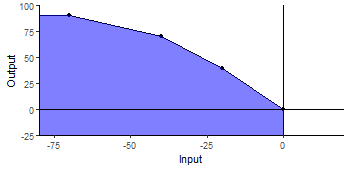
\includegraphics[scale=.75]{problem2b_prodset.png}
	\end{center}
	
	\item[(c)] The largest production set that would rationalize the data is the set that contains all of the observed points, each convex combination of the observed points, the points that would be included if the lines that connected each of the endpoints to their next-closest point in the observed set continued into infinity. The visual representation of the set is provided below.
	
	\begin{center}
	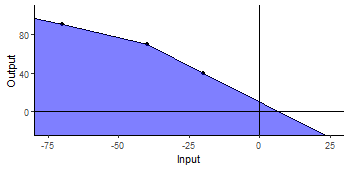
\includegraphics[scale=.75]{problem2c_prodset.png}
	\end{center}
	
\end{itemize}



%%%________________________________________________________________%%%

\section*{Question 3}
\textbf{Suppose you observe only industry-level data at several price vectors of \textit{n} profit-maximizing, price-taking firms. Will this aggregate data satisfy the Weak Axiom of Profit Maximization (WAPM)? Can industry production be rationalized as if it were the choice of a single, profit-maximizing firm?}
\bigskip \\
For $i\in\{1,...,n\}$, let $y_i$ and $Y_i$ denote the production plan and production set, respectively of firm $i$. Since we have $n$ profit-maximizing, price-taking firms, we know that, for $i=\{1,...,n\}$, the WAPM is satisfied:
\[
	p\cdot y_i(p)\geq p\cdot y'_i\text{, where } y_i,y'_i \in Y_i\text{, }p\in\R_+^k
\]
Then, we can prove through induction that WAPM holds for $n$ firms:
\smallskip \\
\indent \textit{Base step}: Let $n=1$. WAPM is trivially satisfied by the assumption that each firm included in the aggregate is profit-maximizing and price-taking.
\smallskip \\
\indent \textit{Induction step}: Assume that WAPM is satisfied for the aggregate of $n$ firms. Let firm $n+1$ be another profit-maximizing, price-taking firm that satisfies WAPM. Then:
\begin{align*}
	p\cdot\left(\sum_{i=1}^{n}y_i(p)\right) 			&\geq p\cdot\left(\sum_{i=1}^{n}y'_i\right)						\\
	p\cdot y_{n+1} + \left(\sum_{i=1}^{n}y_i(p)\right) 	&\geq p\cdot y'_{n+1} + p\cdot\left(\sum_{i=1}^{n}y'_i\right)	\\
	p\cdot\left(\sum_{i=1}^{n+1}y_i(p)\right) 			&\geq p\cdot\left(\sum_{i=1}^{n+1}y'_i\right)					\\
\end{align*}
 Thus, WAPM holds for an arbitrary $n$ firms, where we observe $(\sum_{i=1}^{n}y_i(p))$ as the aggregate industry output. Therefore, if each firm included in the industry aggregate satisfies WAPM, then the industry aggregate will also satisfy WAPM. As a result, the industry aggregate can be rationalized as if it were the output of a single firm.


%%%________________________________________________________________%%%


\end{document}








